\documentclass[11pt]{beamer}
\usetheme{CambridgeUS}
\usepackage[utf8]{inputenc}
\usepackage{amsmath}
\usepackage{amsfonts}
\usepackage{amssymb}
\usepackage{graphicx}

\author{Nico Fröhlich}
\title{Eine Einführung zu graphischen devices}

\setbeamercovered{transparent} 
\setbeamertemplate{navigation symbols}{} 
\institute{Troblecodings} 
\subject{IT}

\begin{document}

\begin{frame}
    \titlepage
\end{frame}

\begin{frame}{Quellen und weiterführende Inhalte}
    \begin{itemize}
        \item Real-Time Rendering - Fourth Edition
        \item Sascha Willems (Github)
        \item Philip Hammer (@philiphammer0)
        \item Physically based rendering
    \end{itemize}
\end{frame}

\begin{frame}{Einführung}
    \begin{itemize}
        \item Berechnen von Matrizen
        \item Primär arithmetisch
        \item Erst seit wenigen Jahren Branching
        \item Bestehen aus vielen Shader Cores
        \item Warps verknüpfen die Cores
    \end{itemize}
\end{frame}

\begin{frame}{Shader Cores}
    \begin{itemize}
        \item 3000 in RTX 2080
        \item Programmierbar
        \item Unabhängig voneinander
        \item Unabhängige Write Locations
        \item Wenig Cache
        \item Keine Branch Prediction
    \end{itemize}
\end{frame}

\begin{frame}{Warps}
    \begin{itemize}
        \item Fassen Cores zusammen
        \item 32 Cores pro Warp
        \item Stall and Swap
        \item SIMD für GPUs
        \item Parallelismus
    \end{itemize}
\end{frame}

\begin{frame}{Warps - Beispiel}
    \begin{figure}[hbtp]
        \centering
        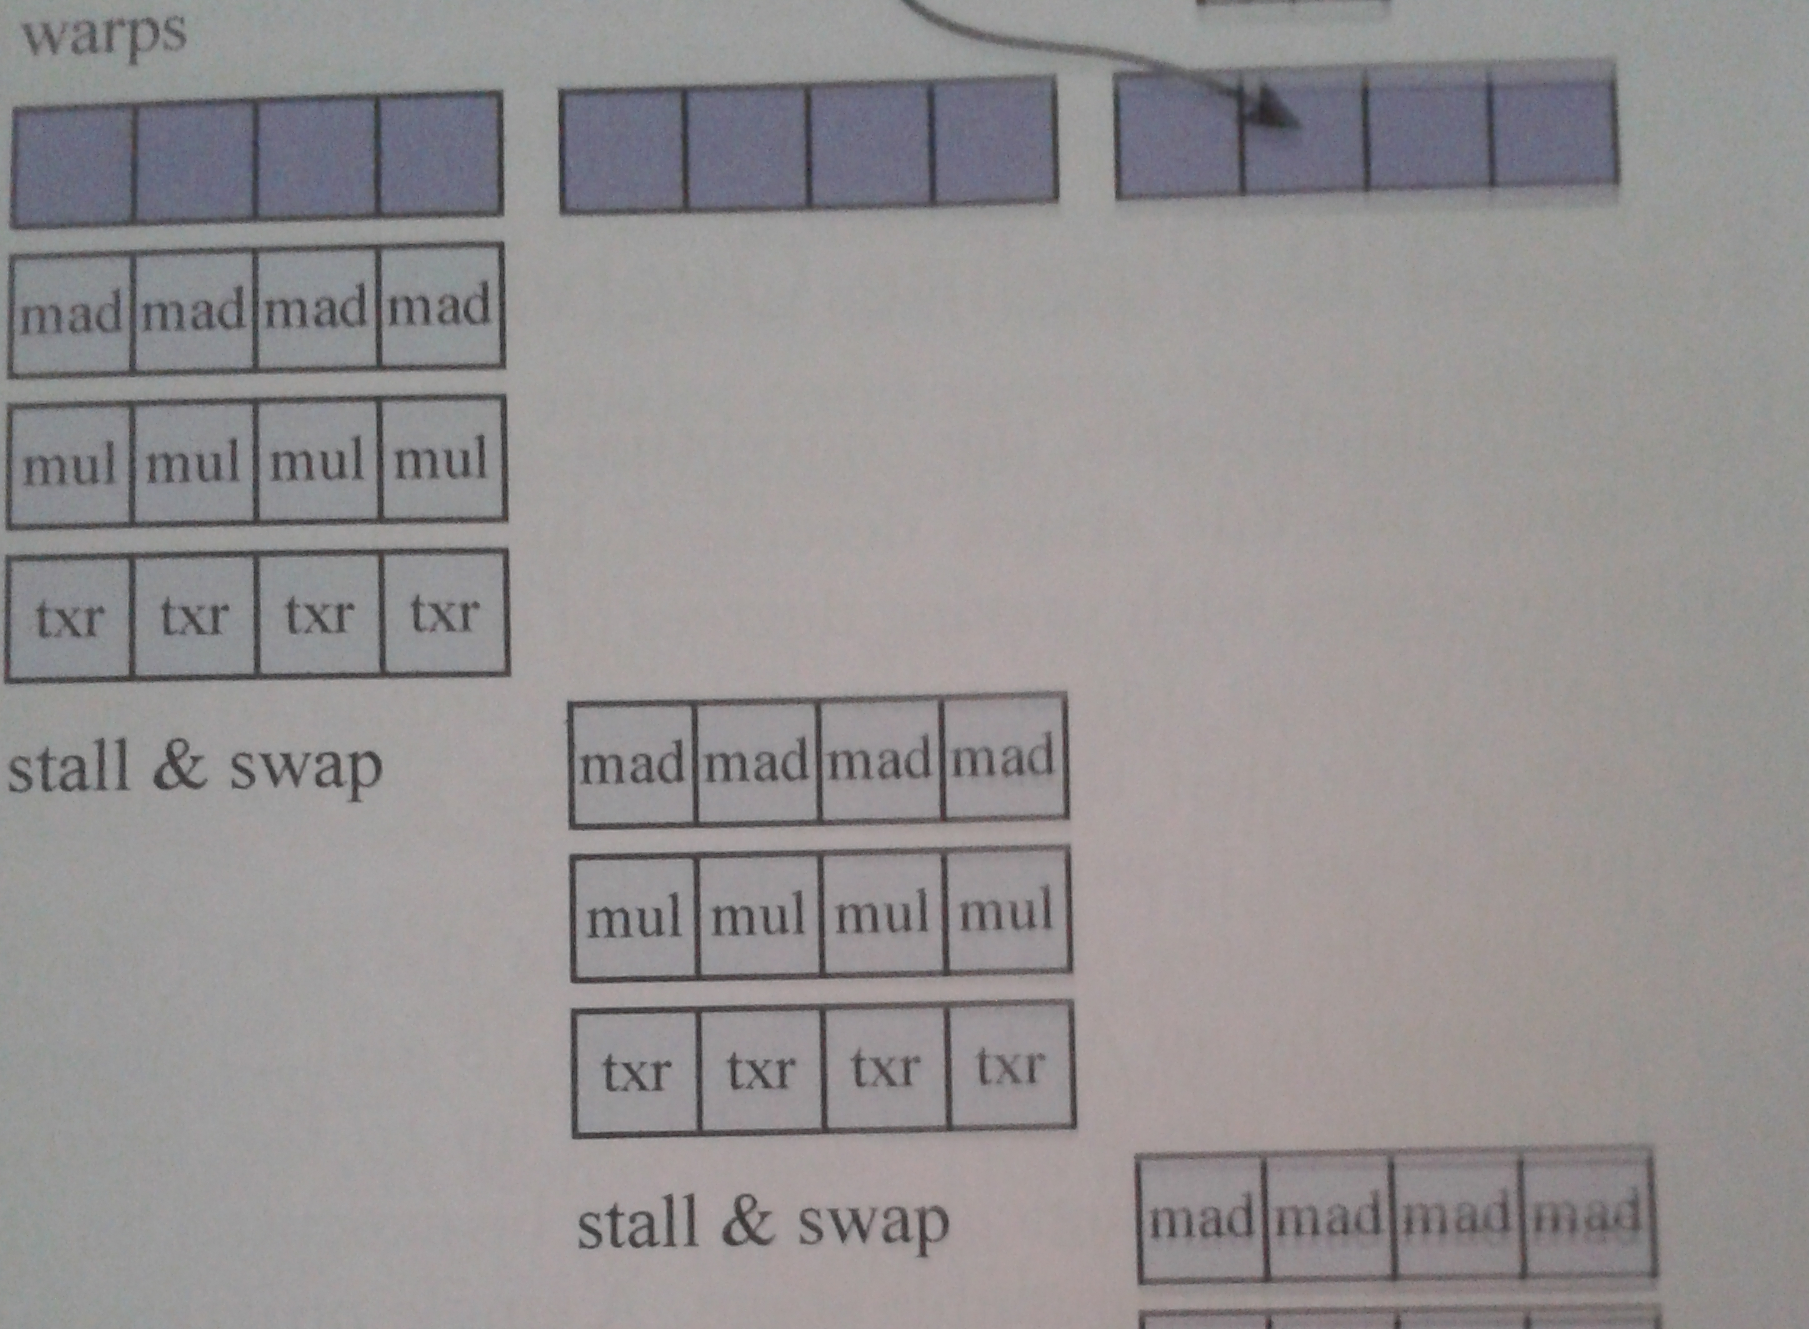
\includegraphics[scale=.14]{swap.png}
        \caption{Stall and Swap}
    \end{figure}
\end{frame}

\begin{frame}{Die Daten}
    \begin{figure}[hbtp]
        \centering
        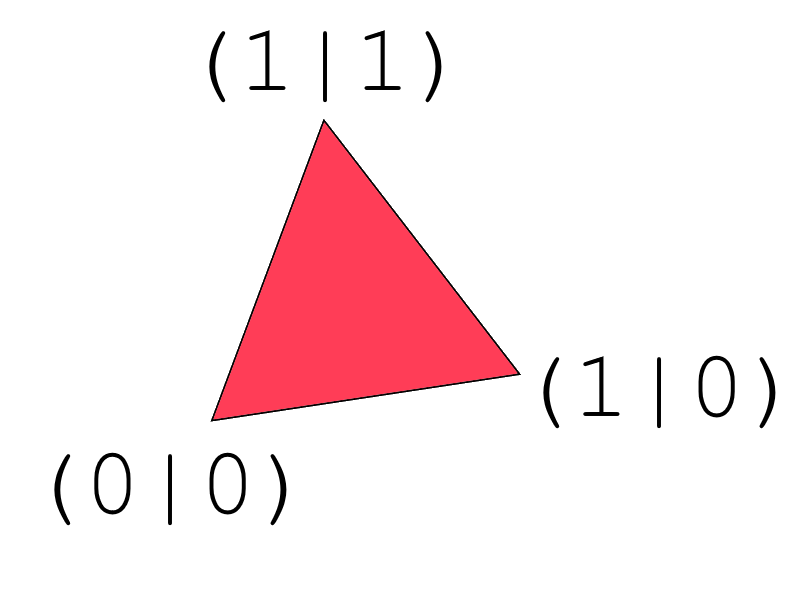
\includegraphics[scale=.4]{data.png}
        \caption{Vertex Daten}
    \end{figure}
\end{frame}

\begin{frame}{Pipelines}
    \begin{figure}[hbtp]
        \centering
        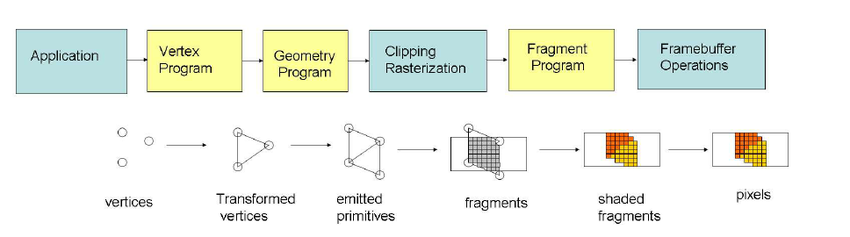
\includegraphics[scale=.4]{pipeline.png}
        \caption{Vertex Daten}
    \end{figure}
\end{frame}

\end{document}
